\documentclass[conference]{IEEEtran}
\usepackage[pdftex]{graphicx}
\usepackage{cite}

% correct bad hyphenation here
\hyphenation{op-tical net-works semi-conduc-tor}

\begin{document}
%
% paper title
% can use linebreaks \\ within to get better formatting as desired
% Do not put math or special symbols in the title.
\title{Multiagent Coordination in Roombas: From the perspective of
    Reinforcement Learning and Neuroevolution}


% author names and affiliations
% use a multiple column layout for up to three different
% affiliations

\author{ 
Jimmy Xin Lin \\
Department of Computer Science\\
the University of Texas at Austin\\
Austin, TX 78712 \\
\texttt{jimmylin@cs.utexas.edu} \\
\and
Barry Feigenbaum \\
The University of Texas at Austin \\
Address \\
\texttt{email} \\
}
% use for special paper notices
%\IEEEspecialpapernotice{(Invited Paper)}

% make the title area
\maketitle

% As a general rule, do not put math, special symbols or citations
% in the abstract
\begin{abstract}
    % aim of this paper
    This paper presents our research about the reinforcement learning approach
    and the neuroevolution approach, by which the crumb collection task can be
    more effectively and efficiently solved with communication and
    coordination between multiple agents under the simulated Roombas
    environment.
    % literature
    The preliminary literature part gives a brief overview about how existing
    works fulfill the coordination under general multiagent environments.
    % results
    The initial setup experimentation shows our works about the
    learned agents that simulate greedy strategies.
    The key things ... are shown in the following multiagent experiments.
    % important conclusion
    It is observed from our experiments that .
\end{abstract}

\IEEEpeerreviewmaketitle



\section{Introduction}
% utility of roomba and some literatures about its usage in real world
In the past years, Roomba Vacuum has gained its popularity in the industry of
domestic services.  Most of existing studies about Roomba (iRobots) is to 
qualitatively investigate its utility in the home as a single autonomous
domestic service provider. In the contrast, our interests focus on the working
efficacy of Roomba agents under a decentralized system.

% Decentralized system
The decentralized decision making has a long history, originated from the team
thoery (\hspace*{-0.85mm} \cite{marschak1955elements, radner1962team,
    radner1959application, ho1972team, tsitsiklis1985complexity}),
where the decisions made by team members need to contribute to the fulfillment
of global objectives. However, the individual members have only partial
information about the entire system, i.e. limited knowledge of common goals
and global states. This motivates the need for coordination because agents
have to share resources and expertise required to achieve their goals.
Researchers in the field of Distributed Artificial Intelligence (DAI) have
been developing efficient mechanisms to coordinate the activities of multiple
autonomous agents (\hspace*{-1.7mm}\cite{weiss1999multiagent, huhns2012distributed}). 
Specifically, previous works for the multiagent coordination 
include using sophisticated information to exchange protocols, investigating
heuristics for negotiation, and developing formal models of possibilities of
conflict and cooperation among agent interests. 

% Reinforcement learning
Reinforcement learning has been widely used as the most useful techniques for
autonomous game playing ( and even Angry Bird) and intelligent task
fulfillment either for single-agent or multi-agent environment. 

% Neuroevolution
Neuroevolution.

% Our aim and contributions in this paper
In this paper, we
investigate various multiagent coordination techniques under the framework of
reinforcemnet learning and neuroevolution could improve the working efficacy
of Roomba in the task of cleaning the floor. 
Our contributions include: 

% outline of this paper
The remained part of this paper is organized as follows. 
In section \ref{section:literature}, a detailed presentation about the
existing  reinforcement learning treatments and the neuroevolution treatments
for multiagent systems.  
Section \ref{section:environment} describes in detail the virtual Roomba
environment, under which our experiments proceed, and the some expected
multi-agent behaviors.  
Preliminary simulations that verify the correct system setup are indicated in
the section \ref{section:setup}. 
We summarize our conclusions and discuss some promising future works in the
section \ref{conclusion}.

\begin{figure}[!t]
\centering
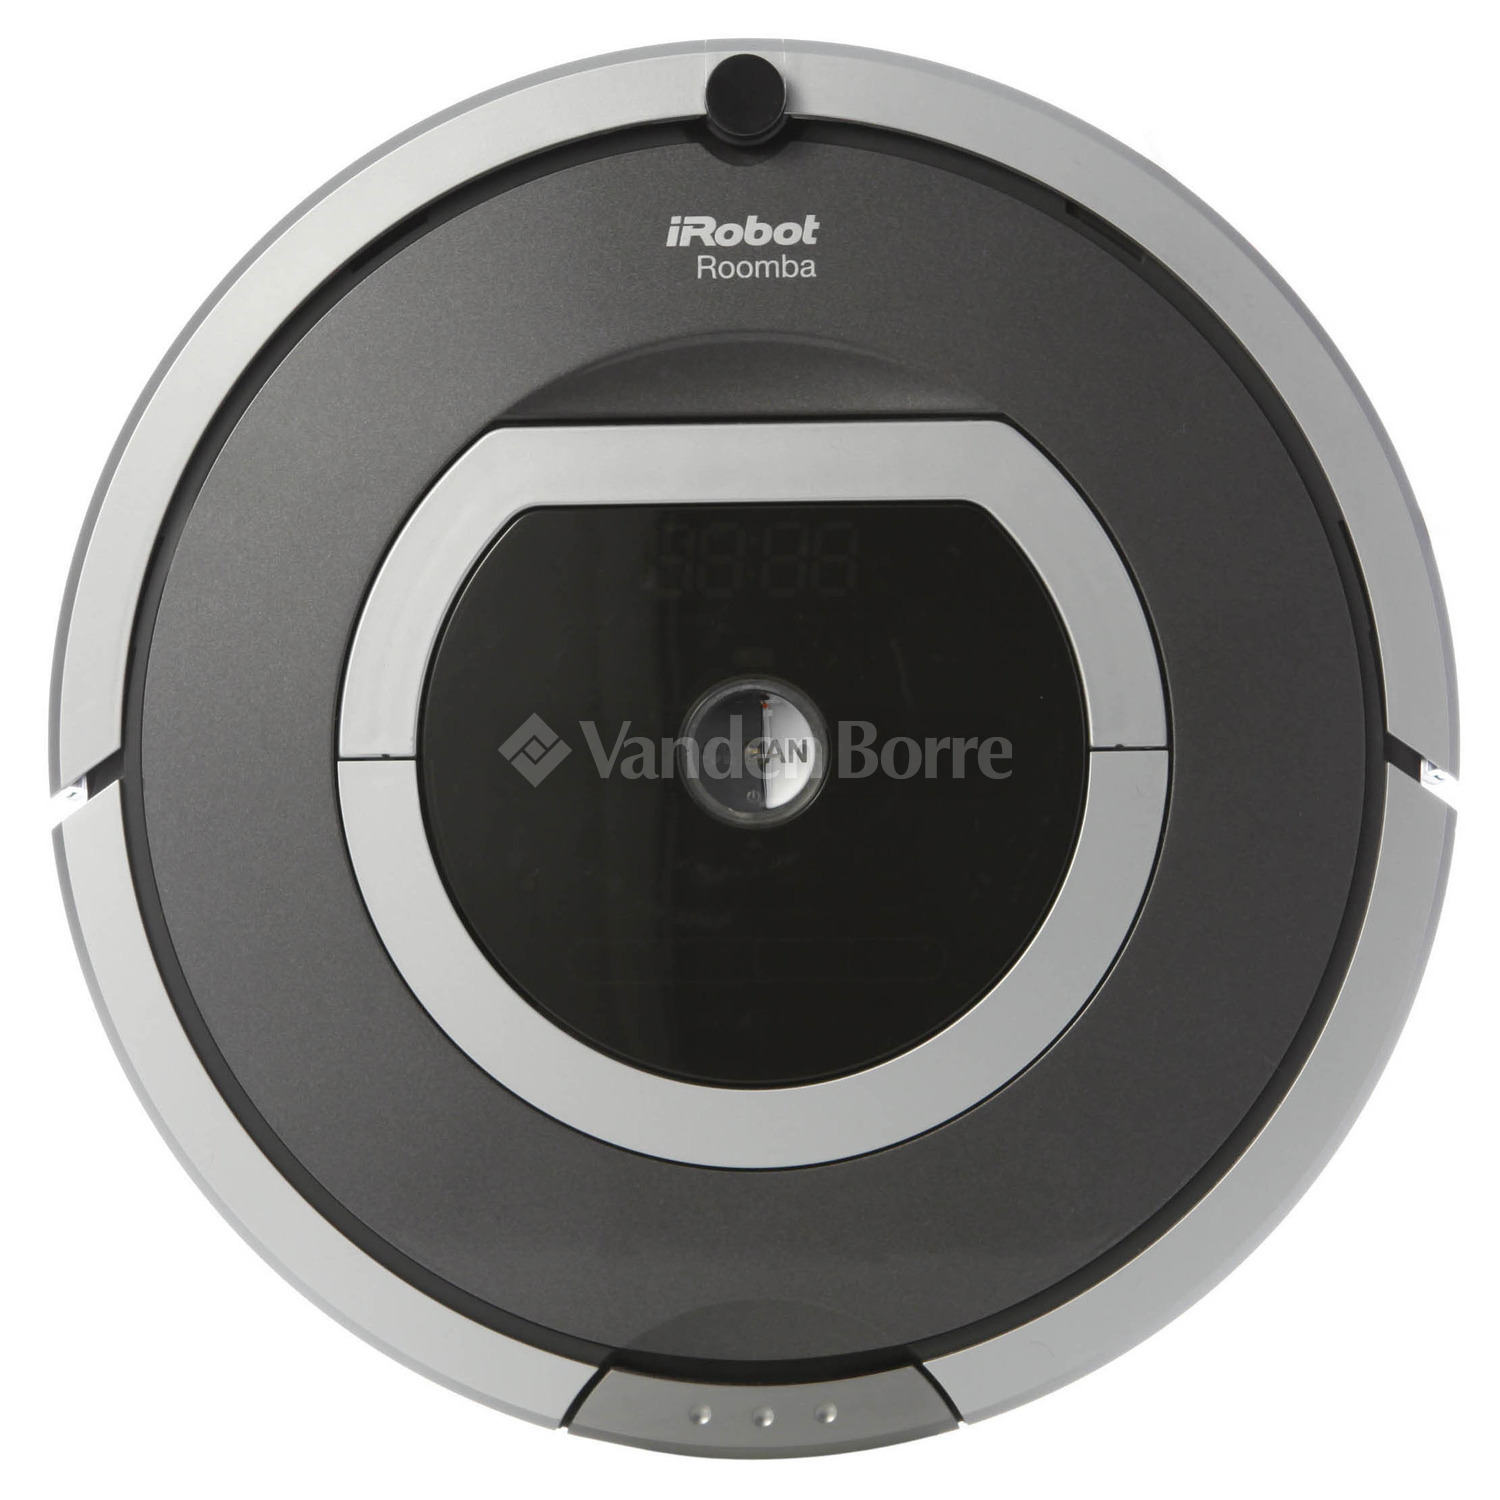
\includegraphics[width=2.1in,height=2.1in]{./figures/irobot_roomba.jpg}
\caption{A exemplar Roomba robot in the real world.}
\label{roomba:world}
\end{figure}


\section{Technical Literatures} \label{section:literature}
This section focuses on the summary of previous works about how multiagent
coordination can be incorporated in the reinforcement learning technique and the
neuroevolution tehnique.
\subsection{Coordinated Multiagent Reinforcement Learning}
\cite{nguyen2014decentralized} Existing work typically assumes that the prob- lem in each time step is decoupled from the problems in other time steps, which might not hold in some applications. Therefore, in this paper, we make the following contributions: (i) We introduce a new model, called Markovian Dynamic DCOPs (MD-DCOPs), where the DCOP in the next time step is a function of the value assignments in the current time step; (ii) We introduce two distributed reinforcement learning algo- rithms, the Distributed RVI Q-learning algorithm and the Dis- tributed R-learning algorithm, that balance exploration and exploitation to solve MD-DCOPs in an online manner; and (iii) We empirically evaluate them against an existing multi- arm bandit DCOP algorithm on dynamic DCOPs.

\cite{zhang2011coordinated} This paper presents a
model-free, scalable learning approach that synthesizes
multi-agent reinforcement learning (MARL) and distributed
constraint optimization (DCOP). By exploiting
structured interaction in ND-POMDPs, our approach
distributes the learning of the joint policy and employs
DCOP techniques to coordinate distributed learning to
ensure the global learning performance. Our approach
can learn a globally optimal policy for ND-POMDPs
with a property called groupwise observability. Experimental
results show that, with communication during
learning and execution, our approach significantly outperforms
the nearly-optimal non-communication policies
computed offline.

SBDO: A New Robust Approach to Dynamic Distributed Constraint Optimisation

\cite{zhang2013coordinating}

\cite{banerjee2012sample}

\cite{kraemer2012informed}

\cite{boukhtouta2011adaptive}
Complex problems involving multiple agents exhibit varying degrees of
cooperation. The levels of cooperation might reflect both differences in
information as well as differences in goals. In this research, we develop a
general mathematical model for distributed, semi-cooperative planning and
suggest a solution strategy which involves decomposing the system into
subproblems, each of which is specified at a certain period in time and
controlled by an agent. The agents communicate marginal values of resources to
each other, possibly with distortion. We design experiments to demonstrate the
benefits of communication between the agents and show that, with
communication, the solution quality approaches that of the ideal situation
where the entire problem is controlled by a single agent.

\cite{sen1994learning}
Researchers in the field of Distributed Artificial
Intelligence (DAI) have been developing efficient
mechanisms to coordinate the activities of multiple
autonomous agents. The need for coordination
arises because agents have to share resources
and expertise required to achieve their goals.
Previous work in the area includes using sophisticated
information exchange protocols, investigating
heuristics for negotiation, and developing
formal models of possibilities of conflict and cooperation
among agent interests. In order to handle
the changing requirements of continuous and
dynamic environments, we propose learning as a
means to provide additional possibilities for effective
coordination. We use reinforcement learning
techniques on a block pushing problem to show
that agents can learn complimentary policies to
follow a desired path without any knowledge
about each other. We theoretically analyze and
experimentally verify the effects of learning rate
on system convergence, and demonstrate benefits
of using learned coordination knowledge on similar
problems. Reinforcement learning based coordination
can be achieved in both cooperative and
non-cooperative domains, and in domains with
noisy communication channels and other stochastic
characteristics that present a formidable c

\subsection{Coordinated Multiagent Neuroevolution}
\textbf{Barry:}
Add literatures of Neuroevolution here...

ATA: barbarian


\section{Simulation Environments} \label{section:environment}
The OpenNERO, an AI research and education platform
\cite{karpov2008opennero}, will be employed for our experimentation.

\subsection{Structure of the Roomba Environment}
% intro to roomba
The Roomba environment is a virtual computer lab with crumbs distributed on
the floor.
In this virtual lab, there are four classes of objects: agents, crumbs, walls,
decorations. 
Vacuum cleaner agents, shown as grey cylinders in Fig. \ref{roomba:world}, are
supposed to collect the static crumbs that are labelled as blue cubes.  
The agents will be rewarded if they move to a place where there are some
crumbs. 
Walls are also set up as the limits of the Roomba environment, such that
agents are not allowed to move beyond the walls and no pellets can be put
outside the walls.
Other decorative objects within the computer lab include tables, chairs, and
computers. For simplicity at the moment, these decorations only serve as
physically transparent decorations, which means they do not block agents' movements.

% controller
As shown in the Fig. \ref{roomba:world}, the small window floating on the top right
is the controller that masters the type of scripted AI agents to load in, the
number of agents, and particular commands that impact the progress of the
Roombas simulation (Pause/Resume, Add/Remove Robots, Exit). On each run of the
simulation, only one particular type of AI agents are allowed to be loaded.
Note also that the type of AI agents employed cannot be switched to the other
one during the intermediate process of crumb collection task. 
If one needs to switch to the other type of AI agents, the running agents have
to be removed and then the user can load the desired AI agents.

%  movement of agents
In the Roombas environment, the movements of vacuum cleaner agents are not
constrained by four directions (left, right, forward, backward). Instead,
agents are able to move towards all directions and each moving action is
denoted as a continuous radius value. Besides, all agents move in a
synchronous way. Agents are allowed to make their movements of the following
step if and only if all agents have completed their movements in the last step.

% placement of pellets 
Three different modes (MANUAL, RANDOM, and CLUSTER) are employed to specify
the placing position of each individual crumb.
In the MANUAL mode, one pellet is deterministically placed at a user-specified
position. 
In the RANDOM mode, the placement of one pellet is totally randomized; the
environment will throw a rejection and repeat the random generation, if an
invalid position is yielded. The last one is the CLUSTER mode, where the
position of pellets are partially randomized. In this mode,
environment samples the position of one pellet from a gaussian distribution
whose centers and spreads at $x$ and $y$ coordinates are specified. 
In this paper, the specifications for the placement of crumbs are generated
from the starting CLUSTER-mode experiment and remained invariant by
employing MANUAL mode in all experiments afterwards.

\begin{figure}[!t]
\centering
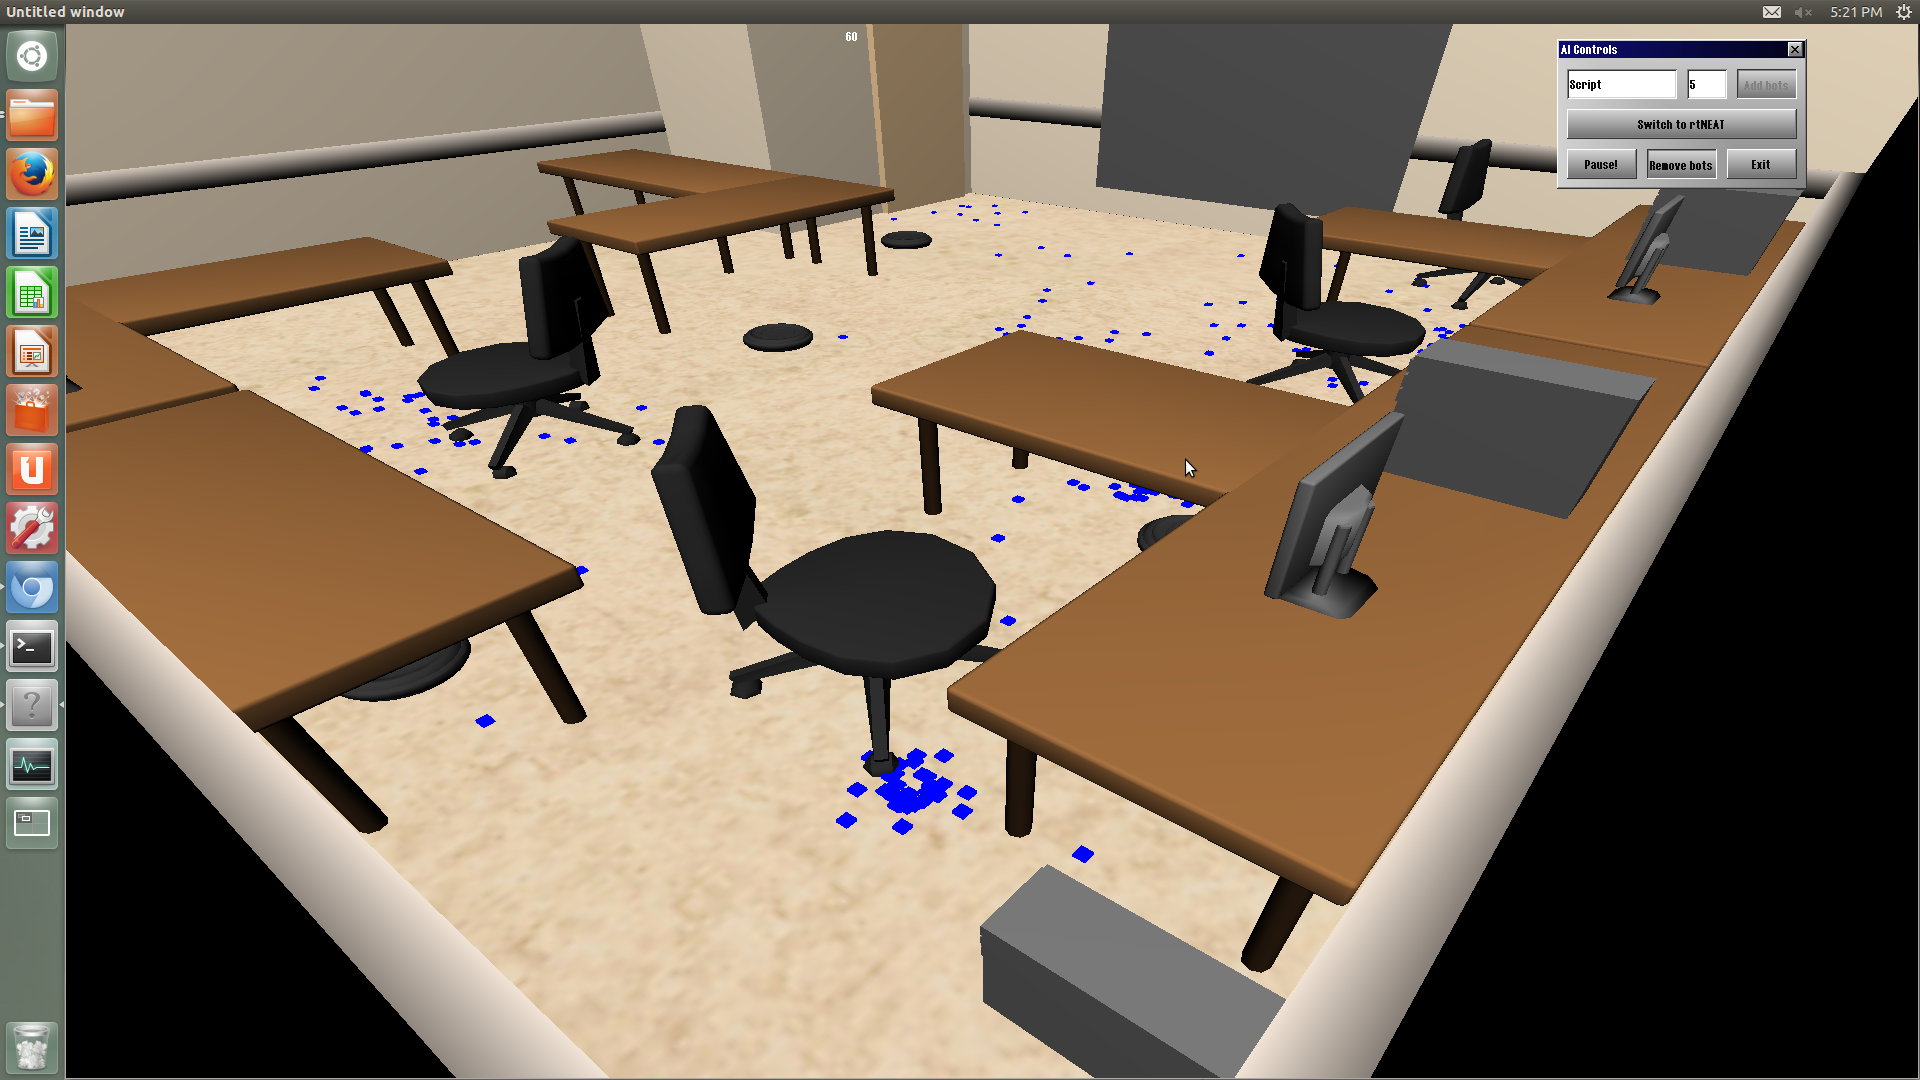
\includegraphics[width=3.2in,height=2.1in]{./figures/roombas/roomba2.png}
\caption{Overall Picture of the Roomba Environment}
\label{roomba:world}
\end{figure}

% sensors (default setting for greedy agents)
The design and representations of sensors have significant impact on the
learning outcome of agents.
Agents are able to perceive limitless information from the computer lab. 
The implementation of Roomba environment allows each agent to sense all crumbs on
the floor about their positions, existence status, and even rewards. In
addition, the spatial information of other vacuum cleaner robots is available
for each individual agent, as well as the user-defined working status of these 
collaborated robots (e.g. a history of previous positions and movements).
Although the Roomba environment provides a large design space for sensors, it
is a practical treatment to start from a small number of
simple sensors. For example, a combination of the bumping status, the position of
its own, and the location of closest crumb suffice for an agent to learn a
greedy strategy, as illustrated in the initial setup experimentation .
A balance is struck between the amount of information available to each agent
and the associated cost.

% rewards
The reward design is another big issue for
configuring the Roomba environment. By default, the only reward being set up
for agents is when they successfully collect some pellets on the floor. In
order to facilitate the learning of agents, an penalty for being alive is
supposed to be incorporated to the reward system. That is, agents should
receive some negative rewards, typically a very small quantity, for each step
they move. Similarly, penalties can also be granted to the collisions between
roombas, bumping of agents towards the world boundaries, and repetitive
movements around an area.


\subsection{Expected Multiagent Behaviors}
Work Balance / competition avoidance. 

Collision avoidance. 


\section{Experiments: Initial Setup} \label{section:setup}
This section will present some preliminary results coming from the simulation
of greedy agents. Agents with greedy strategy simply approaches to the direction
where the closest pellet to it is there.  These results may not be directly
related to the multiagent behaviors, but 
(i) demonstrate that we have set up the environment correctly for both
of the reinforcement learning technique and the neuroevolution technique. 
(ii) illustrate intuitively the benchmark intelligence for the crumb
collection.

\subsection{Reinforcement Learning}
Add implementation details of Q-Learning and variants here...

\subsection{Neuroevolution}
\textbf{Barry:}
Add implementation details of Neuroevolution here...

\section{Experiments: Multiagent Coordination}
After the experimentation for testing the initial setup of Roombas
environment, the intention of this section is to investigate the problem of
how to incorporate effective coordinations for this particular multiagent
system.
\subsection{Reinforcement Learning}

\subsection{Neuroevolution}

%\begin{figure}[!t]
%\centering
%\includegraphics[width=2.5in]{myfigure}
%\caption{Simulation Results.}
%\label{fig_sim}
%\end{figure}



\section{Conclusions} \label{conclusion}
The conclusion goes here. 

Future Works go here.

% trigger a \newpage just before the given reference
% number - used to balance the columns on the last page
% adjust value as needed - may need to be readjusted if
% the document is modified later
%\IEEEtriggeratref{8}
% The "triggered" command can be changed if desired:
%\IEEEtriggercmd{\enlargethispage{-5in}}

% references section

% can use a bibliography generated by BibTeX as a .bbl file
% BibTeX documentation can be easily obtained at:
% http://www.ctan.org/tex-archive/biblio/bibtex/contrib/doc/
% The IEEEtran BibTeX style support page is at:
% http://www.michaelshell.org/tex/ieeetran/bibtex/

\bibliographystyle{IEEEtran}
\bibliography{report}

% <OR> manually copy in the resultant .bbl file
% set second argument of \begin to the number of references
% (used to reserve space for the reference number labels box)

%\begin{thebibliography}{1}
%\bibitem{IEEEhowto:kopka}
%H.~Kopka and P.~W. Daly, \emph{A Guide to \LaTeX}, 3rd~ed.\hskip 1em plus
%  0.5em minus 0.4em\relax Harlow, England: Addison-Wesley, 1999.
%\end{thebibliography}




% that's all folks
\end{document}
